\section{Classification}

\subsection{Nearest Neighbour}

The \acrfull{KNN} algorithm is an example of instance based learning and works by extracting a set of features for each sample and using this `feature vector' to represent each sample in a multidimensional vector space.

Once this space has been generated, new samples may be classified by generating their feature vector and calculating the $k$ closest or `most similar' samples in the model by way of a distance calculation. By considering the $k$ closest samples, a consensus can be reached and the new sample is classified according to the label with the greatest majority in the $k$ nearest neighbours as seen in \cref{fig:knn-example}.

 \begin{figure}[h!]
   \centering
   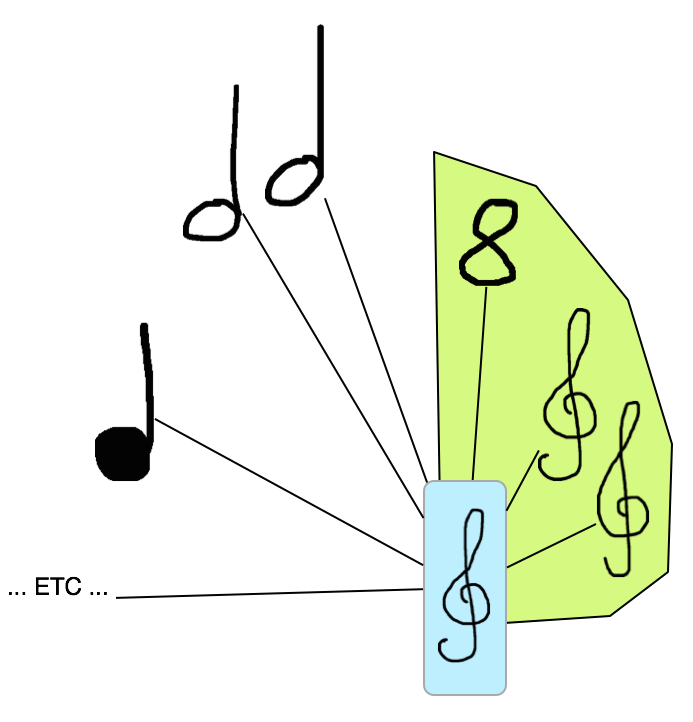
\includegraphics{gfx/techniques/knn-entities.png}
   \caption{KNN example using musical symbols and a K value of 3. The new symbol being classified is highlighted blue and the three closest three entities in green. In this case, the sample would be classified as a treble clef}
   \label{fig:knn-example}
 \end{figure}

The two most critical aspects of the KNN classifier are the distance method used and the number of neighbours considered. In order to maximise the accuracy of the classifier, I performed several experiments to this effect in \cref{sec:implementation-classification}.

\subsection{KNN Editing}

Although KNN can produce good results, the need to store all the data makes it less attractive. To reduce the data needed in classifiers you can use an edited KNN algorithm where the idea is to try and remove ``poor" samples which not only reduces the storage requirements but should also improve the accuracy of the classifier.

\subsubsection{Wilson Editing}
I originally came across the idea of edited KNN classifiers in \cite{fujinaga1996adaptive} in which he outlines the original KNN editing techniques from earlier work by \cite{wilson1972asymptotic}, (the algorithm for this editing technique is outlined in \cref{alg:knn-edit}). You can further extend the algorithm to multiple iterations (referred to by most as the multi-editing algorithm), repeating the process until no more poor samples are removed, at which point you save the model for use in classification, hopefully at a reduced dataset size.

\begin{algorithm}[H]
  \caption{KNN editing algorithm}
  \label{alg:knn-edit}

  \begin{algorithmic}
    \Procedure{EditModel}{model}
        \State trainingSamples = \Call{GetSamples}{model}
        \For {each sample in trainingSamples}
          \State classification = \Call{model.classify}{sample}
          \If{classification $\neq$ sample.classification}
            \Call{removeSample}{sample}
          \EndIf
    	\EndFor
    \EndProcedure
  \end{algorithmic}
\end{algorithm}

\subsubsection{Genetic Algorithms}

Although I decided not to actually employ the use of genetic algorithms in this project, they came up repeatedly in more recent research and so I felt it was worth mentioning. Genetic algorithms for feature selection is nothing new, indeed it's used in \cite{fujinaga1996adaptive} for selecting which features to use in a classifier; a traditionally tricky problem when you have lots of features (or indeed classifier variables such as the value of K in KNN classification) and need to work out which ones actually produce the best division of classes. Though there are other techniques to do this too like PCA\footnote{Principal Component Analysis is used to find the dimension/variable in a feature vector which provides the highest variance possible. Features which provide small variance are of little help in a classification problem}. However in \cite{kuncheva1995editing} it is used specifically in editing a KNN classifier. The results suggested that it might perform comparably to wilson's technique and that it generally performed better than just using a random sample training set but relative to multi-editing technique the authors state that the results from genetic algorithm and multi editing could not be compared due to an inability to properly evaluate the power of the multi-edit algorithm.